\documentclass[a4paper,14pt]{extreport}
\usepackage[left=1.5cm,right=1.5cm,
    top=1.5cm,bottom=2cm,bindingoffset=0cm]{geometry}
\usepackage{scrextend}
\usepackage[T1,T2A]{fontenc}
\usepackage[utf8]{inputenc}
\linespread{1.5}
\usepackage[english,russian,ukrainian]{babel}
\usepackage{tabularx}
\usepackage{amssymb}
\usepackage{color}
\usepackage{amsmath}
\usepackage{mathrsfs}
\usepackage{listings}
\usepackage{graphicx}
\graphicspath{ {./images/} }
\usepackage{lipsum}
\usepackage{xcolor}
\usepackage{hyperref}
\usepackage{tcolorbox}
\usepackage{tikz}
\usepackage[framemethod=TikZ]{mdframed}
\usepackage{wrapfig,boxedminipage,lipsum}
\mdfdefinestyle{MyFrame}{%
linecolor=blue,outerlinewidth=2pt,roundcorner=20pt,innertopmargin=\baselineskip,innerbottommargin=\baselineskip,innerrightmargin=20pt,innerleftmargin=20pt,backgroundcolor=gray!50!white}
 \usepackage{csvsimple}
 \usepackage{supertabular}
\usepackage{pdflscape}
\usepackage{fancyvrb}
%\usepackage{comment}
\usepackage{array,tabularx}
\usepackage{colortbl}
\usepackage{fp}

\usepackage{varwidth}
\tcbuselibrary{skins}
\usepackage{fancybox}


\usepackage{tikz}
\usepackage[framemethod=TikZ]{mdframed}
\usepackage{xcolor}
\usetikzlibrary{calc}
\makeatletter
\newlength{\mylength}
\xdef\CircleFactor{1.1}
\setlength\mylength{\dimexpr\f@size pt}
\newsavebox{\mybox}
\newcommand*\circled[2][draw=blue]{\savebox\mybox{\vbox{\vphantom{WL1/}#1}}\setlength\mylength{\dimexpr\CircleFactor\dimexpr\ht\mybox+\dp\mybox\relax\relax}\tikzset{mystyle/.style={circle,#1,minimum height={\mylength}}}
\tikz[baseline=(char.base)]
\node[mystyle] (char) {#2};}
\makeatother

\definecolor{ggreen}{rgb}{0.4,1,0}
\definecolor{rred}{rgb}{1,0.1,0.1}
\definecolor{amber}{rgb}{1.0, 0.75, 0.0}
\definecolor{babyblue}{rgb}{0.54, 0.81, 0.94}
\definecolor{amethyst}{rgb}{0.6, 0.4, 0.8}

\usepackage{float}
\usepackage{wrapfig}
\usepackage{framed}
%for nice Code{
\lstdefinestyle{customc}{
  belowcaptionskip=1\baselineskip,
  breaklines=true,
  frame=L,
  xleftmargin=\parindent,
  language=C,
  showstringspaces=false,
  basicstyle=\small\ttfamily,
  keywordstyle=\bfseries\color{green!40!black},
  commentstyle=\itshape\color{purple!40!black},
  identifierstyle=\color{blue},
  stringstyle=\color{orange},
}
\lstset{escapechar=@,style=customc}
%}


\begin{document}
\pagecolor{white}

%----------------------------------------1
\newtcbox{\xmybox}[1][red]{on line, arc=7pt,colback=#1!10!white,colframe=#1!50!black, before upper={\rule[-3pt]{0pt}{10pt}},boxrule=1pt, boxsep=0pt,left=6pt,right=6pt,top=2pt,bottom=2pt}



\begin{titlepage}
  \begin{center}
    \large
    Національний технічний університет України \\ "Київський політехнічний інститут імені Ігоря Сікорського"


    Факультет Електроніки

    Кафедра мікроелектроніки
    \vfill

    \textsc{ЗВІТ}\\

    {\Large Про виконання лабораторної роботи №1\\
      з дисципліни: «Твердотільна електроніки-2»\\[1cm]

      «ДОСЛІДЖЕННЯ ДИФУЗІЙНИХ РЕЗИСТОРІВ ІНТЕГРАЛЬНИХ МІКРОСХЕМ» \\

    }
  \bigskip
\end{center}
\vfill

\newlength{\ML}
\settowidth{\ML}{«\underline{\hspace{0.4cm}}» \underline{\hspace{2cm}}}
\hfill
\begin{minipage}{1\textwidth}
Виконавець:\\
Студент 3-го курсу \hspace{4cm} $\underset{\text{(підпис)}}{\underline{\hspace{0.2\textwidth}}}$  \hspace{1cm}А.\,С.~Мнацаканов\\
\vspace{1cm}

Перевірив: \hspace{6.1cm} $\underset{\text{(підпис)}}{\underline{\hspace{0.2\textwidth}}}$  \hspace{1cm}Л.\,М.~Королевич\\

\end{minipage}

\vfill

\begin{center}
2021
\end{center}
\end{titlepage}
%---------------------------------------------------------------------------------------------------------------------------------------------------------------------------------



\begin{center}1. МЕТА РОБОТИ\\ \end{center}

Вивчення будови та основних характеристик дифузійних резисторів інтегральних
мікросхем.

\begin{center}2. ЗАВДАННЯ\\ \end{center}\par

2.1 Виміряти вольт-амперні характеристики 5...7 резисторів запропонованої інтегральної
мікросхеми (рис.1) одним із методів.\\

2.2 Дослідити амплітудно-частотну характеристику коефіцієнта передачі схеми із
дифузійним резистором в якості нагрузки - $K_{d}(f)= E_{\text{вих}}/E_{\text{вх}}$ .\\

2.3 За результатами вимірювань побудувати графіки: вольт-амперних характеристик
досліджених резисторів; залежностей коефіцієнта передачі схеми із дифузійним
резистором та загального опору дифузійного резистора від частоти — $K_{d}$(IgF), $Z_{d}$(IgF).\\

2.4 Вирахувати номінальні опори $R_{H-ij}$ дифузійних резисторів.\\


2.5 Пояснити залежність опору дифузійного резистора від напруги, температури і частоти
вимірювального сигналу. Провести аналіз паразитних зв'язків дифузійного резистора.\\

2.6 Запропонувати способи зменшення чи ліквідування впливу паразитної ємності та
паразитного транзистора на роботу дифузійного резистора.

\newpage
\begin{center}3. СХЕМА ДЛЯ ДОСЛІДЖЕННЯ ВОЛЬТ-АМПЕРНОЇ ХАРАКТКРИСТИКИ\\ \end{center}

\begin{figure}[ht]
\center{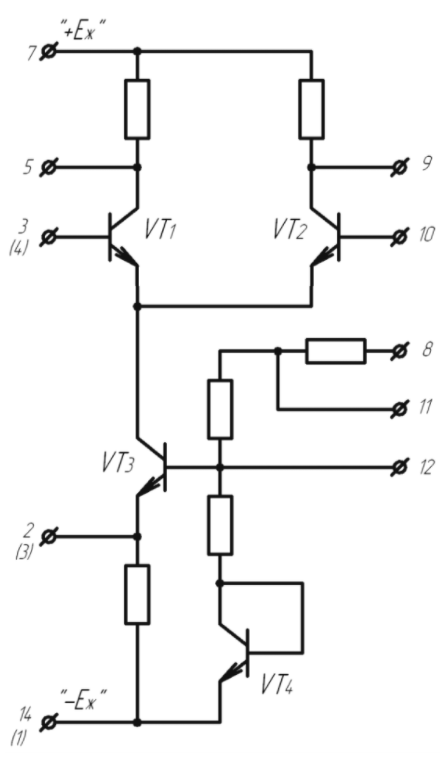
\includegraphics[width=0.4\linewidth]{1.png}}
\caption{Схема вимірювання.}
\label{ris111}
\end{figure}
\newpage


\begin{center}4.Результати вимірювань\end{center}

\begin{figure}[h!]
\center{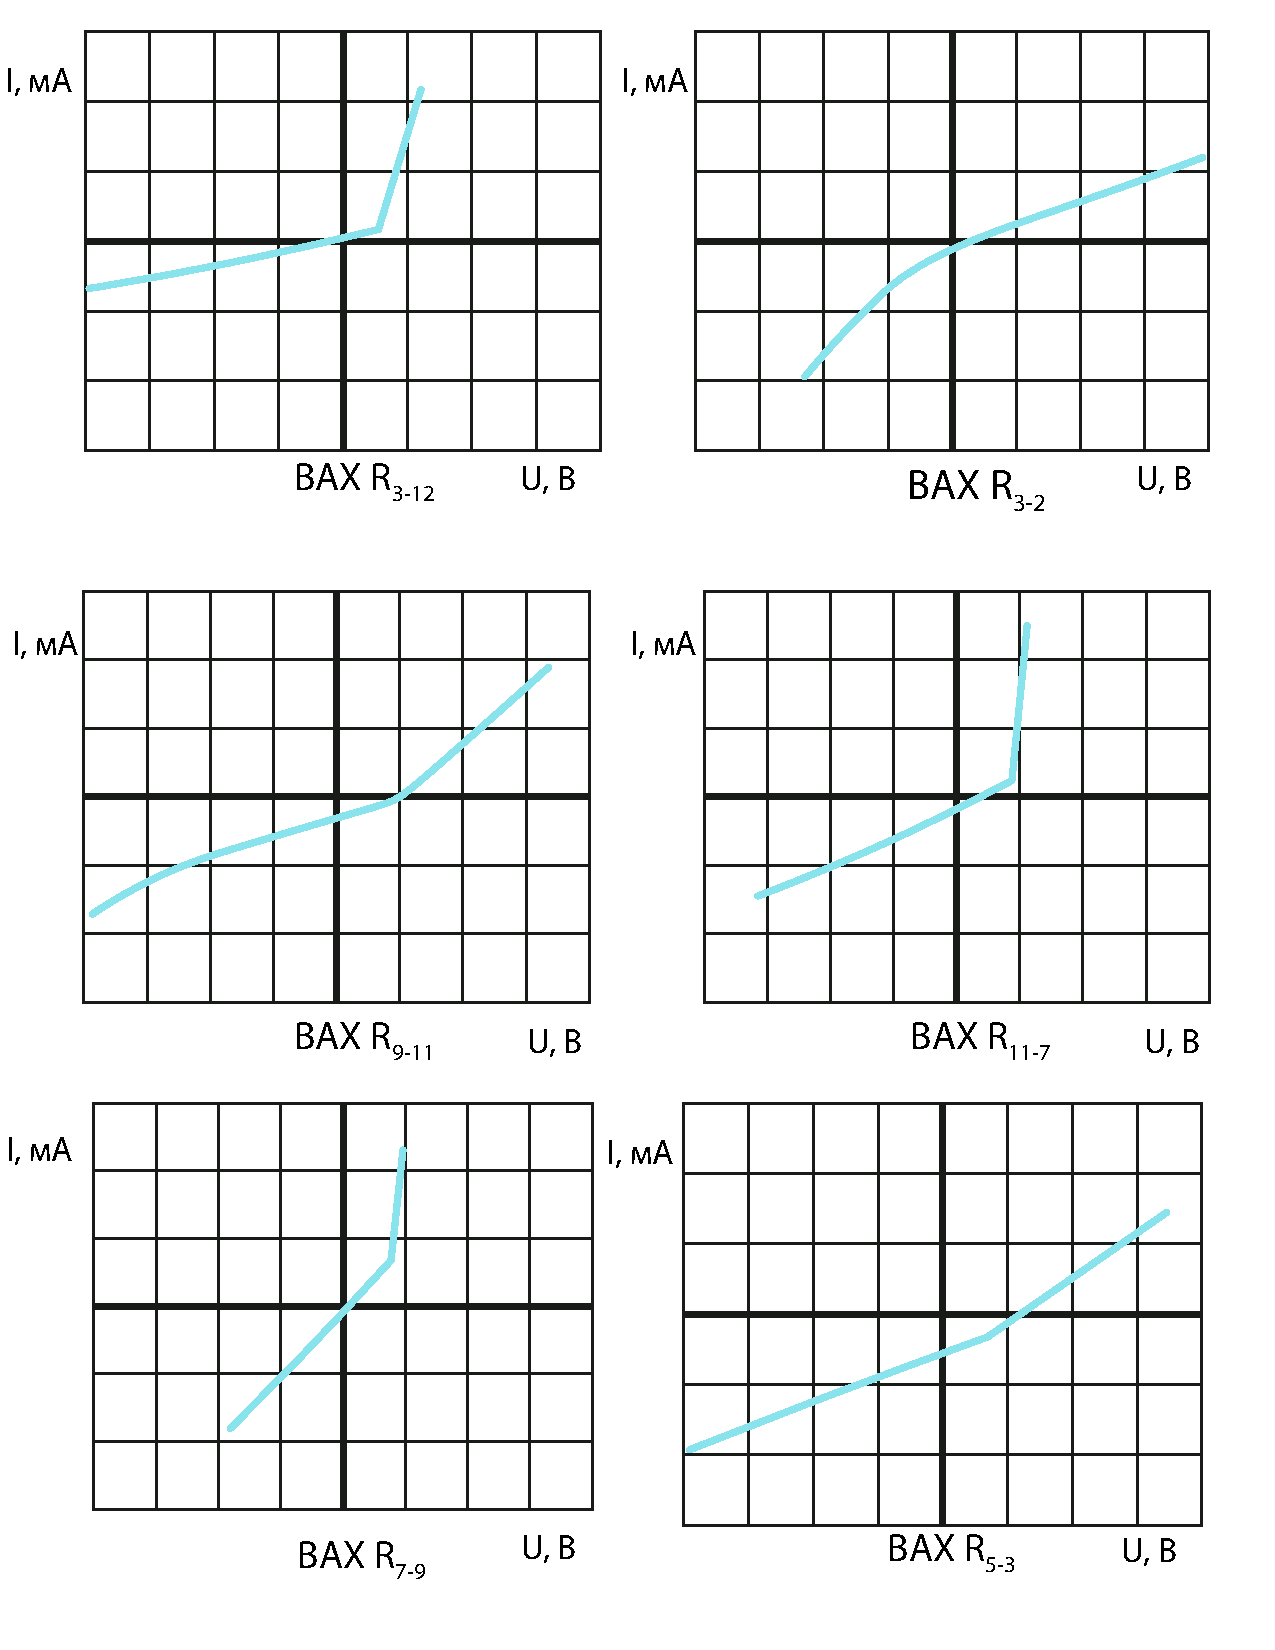
\includegraphics[width=1\linewidth]{111.pdf}}
\end{figure}


\begin{figure}[h!]
\center{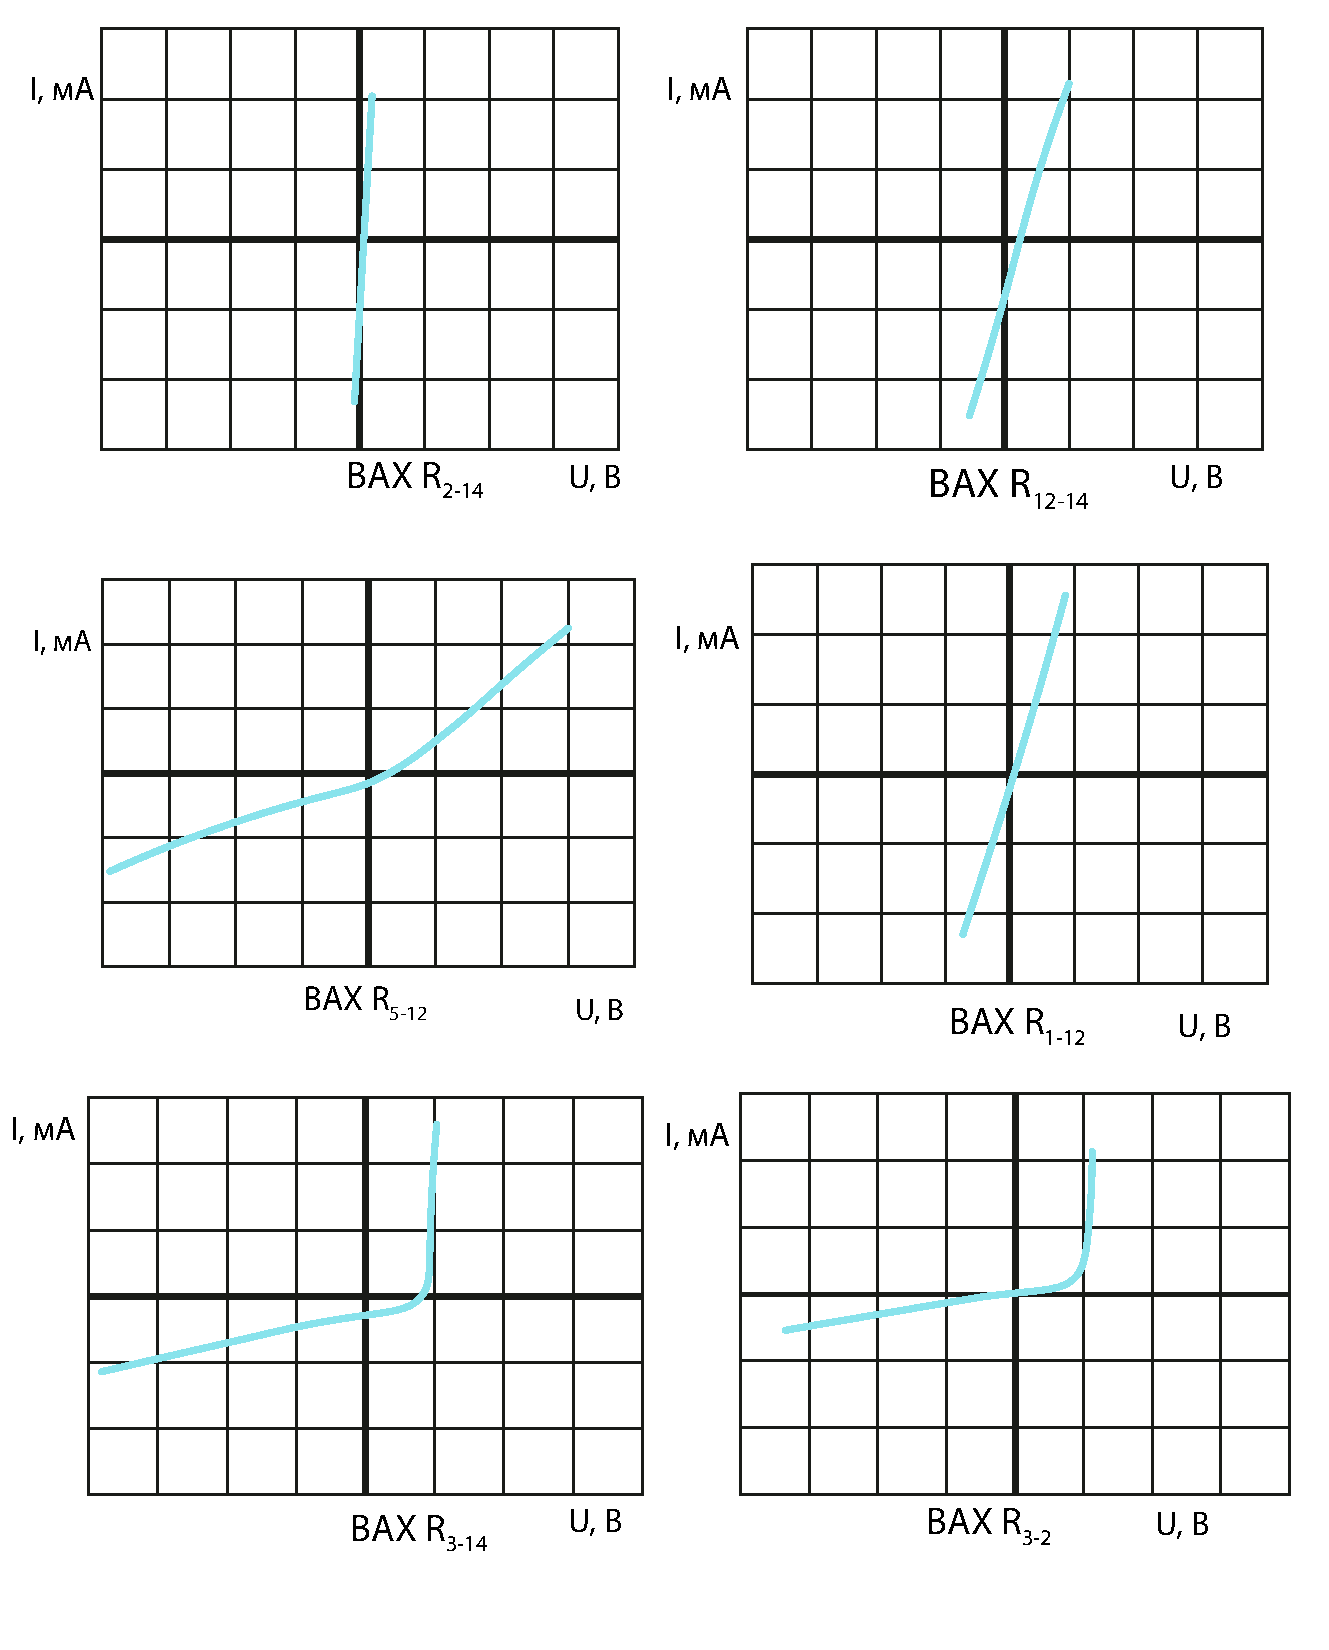
\includegraphics[width=0.9\linewidth]{222.pdf}}
\end{figure}

\clearpage




\begin{center}3.Формули та Розрахунки\\ \end{center}

\FPeval\ra{   round((0.015/(0.0008*10^{-3})):1)   }
$$ R_{3-12} = \dfrac{0,015}{0,0008\cdot 10^{-3}} = \FPprint\ra \approx 18 \text{ кОм}$$
\FPeval\raa{   round((0.01/(0.00012*10^{-3})):1)   }
$$ R_{3-2} = \dfrac{0,01}{0,00012\cdot 10^{-3}} = \FPprint\raa \approx 83 \text{ кОм}$$
\FPeval\raaa{   round((0.01/(0.0008*10^{-3})):1)   }
$$ R_{9-11} = \dfrac{0,01}{0,0008\cdot 10^{-3}} = \FPprint\raaa \approx 12 \text{ кОм}$$
\FPeval\rb{   round((0.01/(0.0004*10^{-3})):1)   }
$$ R_{11-7} = \dfrac{0,01}{0,0004\cdot 10^{-3}} = \FPprint\rb \approx 25 \text{ кОм}$$
\FPeval\rbb{   round((0.01/(0.0004*10^{-3})):1)   }
$$ R_{7-9} = \dfrac{0,01}{0,0004\cdot 10^{-3}} = \FPprint\rbb \approx 25 \text{ кОм}$$
\FPeval\rbbb{   round((0.02/(0.0008*10^{-3})):1)   }
$$ R_{5-3} = \dfrac{0,02}{0,0008\cdot 10^{-3}} = \FPprint\rbbb \approx 25 \text{ кОм}$$



\FPeval\rc{   round((0.002/(0.0002*10^{-3})):1)   }
$$ R_{2-14} = \dfrac{0,002}{0,0002\cdot 10^{-3}} = \FPprint\rc \approx 10 \text{ кОм}$$
\FPeval\rcc{   round((0.01/(0.0002*10^{-3})):1)   }
$$ R_{12-14} = \dfrac{0,01}{0,0002\cdot 10^{-3}} = \FPprint\rcc \approx 50 \text{ кОм}$$
\FPeval\rccc{   round((0.01/(0.0006*10^{-3})):1)   }
$$ R_{5-12} = \dfrac{0,01}{0,0006\cdot 10^{-3}} = \FPprint\rccc \approx 16 \text{ кОм}$$
\FPeval\rd{   round((0.015/(0.0002*10^{-3})):1)   }
$$ R_{1-12} = \dfrac{0,015}{0,0002\cdot 10^{-3}} = \FPprint\rd \approx 75 \text{ кОм}$$
\FPeval\rdd{   round((0.01/(0.0004*10^{-3})):1)   }
$$ R_{3-14} = \dfrac{0,01}{0,0004\cdot 10^{-3}} = \FPprint\rdd \approx 25 \text{ кОм}$$
\FPeval\rddd{   round((0.01/(0.0004*10^{-3})):1)   }
$$ R_{3-2} = \dfrac{0,01}{0,0004\cdot 10^{-3}} = \FPprint\rddd \approx 25 \text{ кОм}$$




















\clearpage
\begin{center}5. Висновок\\ \end{center}

В даній лабораторній роботі було виміряно вольт-амперні характеристики дифузійних резисторів заданої інтегральної мікросхеми, після чого з отриманих ВАХ було розраховано номінальні опори дифузійних резисторів. Також хочу зазначити, що  при додаванні шарів p та n типу до дифузійного транзистора, буде утворюватися паразитний транзистор, для подавлення якого подають зворотно зміщену напруга на n-область транзистора. Наскільки великою може бути напруга для інтегрального резистора, визначає напруга пробою ізолюючого p-n переходу.



\end{document}
